\chapter{Investigating the Blockchain Technology
  in the Context of Cybersecurity}
\markboth{Investigating the Blockchain Technology
	in the Context of Cybersecurity}{}
\chaptauthors{Lenz, Pascal, Roland, Silas}

\Kurzfassung{
The ability of the blockchain technology to handle tasks in a decentralized manner and its property to leave an audit trail of all its history makes it a perfect match when addressing cyber security related issues. Wether it directly mitigates them or it is used to create more secure applications, the blockchain has a lot to offer. This paper starts with a brief introduction to blockchains in general and continues with an overview of the various approaches and ideas that exist for the integration of the blockchain technology into the applications to increase overall security of the application or a whole scenario.}



TODOs:
Shortening and finalizing till monday
Important: CHECK your bibtex entries
\begin{enumerate}
	\item Introduction: 1 - 2 pages --> Roland
	\item Background all together max 6 pages (2 pages each)
	\item Related work max 6 pages per chapter
	\item Conclusion: 2 pages --> Silas
\end{enumerate}


\newpage

\minitoc %table of contents

\newpage
\section{Introduction}

Since the initial development of computing and communication systems, their security has been an ever-growing concern. More and more data is being collected and shared between entities and third-parties \citep{Plageras2017}. Protecting this data and the underlying systems is of utmost importance for our internet-based economy, as companies are bound by increasingly strict laws and need their customers to be confident in data privacy.

The evolution of Blockchain systems over the past decade has led to research on a broad range of application areas in computer science as well as other contexts. Amongst many others, the applications of Blockchain technologies to secure systems and data has been an area of very recent research \citep{Huckle2016}. The primary goal of this work is, therefore, to provide an overview of key areas where such technologies could be applied in future systems.

To establish a solid foundation, Section~\ref{sec:02_background} provides a summary of the most important basic concepts and technical background. More specifically, Section~\ref{subsec:02_cybersecurity} goes into the traditional concepts of cybersecurity and the threat models that have been developed in the area (\textit{e.g.}, the CIA triangle~\cite{whitman2011principles}). Section \ref{subsec:02_Blockchain} then presents the basics of Blockchain on the example of Bitcoin, while Section \ref{subsec:02_smart_contracts} summarizes the concept of smart contracts, an evolution based on the core infrastructure of the Blockchain.

On a lower, more technical level, this work focuses on the applications of Blockchain for the prevention of Distributed Denial of Service (DDoS) attacks, as well as the improvement of critical parts of the internet infrastructure. DDoS attacks are a possibility for attackers to flood the service of a company. Such attacks can lead to availability issues (\textit{e.g.}, causing service downtimes) and thus result in significant business forfeits. Approaches to protecting networks against such DDoS attacks using Blockchain technologies are summarized in Section~\ref{subsec:03_ddos}.

A critical part of the internet and communications security in today's environment is the existence of communication methods that participants trust to deliver messages securely and confidently. Public Key Infrastructures (PKI) provide the backbone for many of these methods. Existing PKI architectures often rely on a centralized infrastructure, which enables many kinds of attacks. We provide an overview of possible improvements to PKI using Blockchain technologies in Section \ref{subsec:03_pki}.

The emergence of the Internet of Things (IoT) and a growing market for interconnected devices brings exciting challenges for Blockchain use. Section \ref{subsec:03_IoT} reviews some of the most critical security and privacy challenges, as well as how they can be mitigated with Blockchain technology. It provides an overview of how Blockchain can help with proving the integrity of IoT data (\textit{e.g.}, smart meters) and goes into how Blockchain can strengthen the security of IoT in the current state of research (\textit{e.g.}, in smart homes).

The goal of this report is not only to cover theoretical concepts or frameworks but also to shed some light on existing real-world applications or proposed system architectures that are currently being developed (presented in Section~\ref{subsec:03_applications}). These applications show us whether the theoretical concepts apply to the real world as well as what types of problems and issues arise.


\newpage
\section{Background}
\label{sec:02_background}

In this section, we build a foundation with regards to the theoretical concepts and background that are needed to follow the concepts presented in section \ref{sec:03_related_work}. First Section \ref{subsec:02_cybersecurity} presents the traditional ideas of cybersecurity as they have been part of research for the past decades. Subsequently, Section \ref{subsec:02_blockchain} elaborates on the core concepts of the blockchain which are necessary to understand the main research topic of this work. Finally, Section \ref{subsec:02_smart_contracts} reviews the concept of smart contracts and how they have developed as an evolution of the existing blockchain architecture.

\subsection{Cybersecurity}
\label{subsec:02_cybersecurity}

Cybersecurity has the potential to be one of the most global interests for governmental or private institutions, as well as for individuals. Political, financial, corporate, military, and medical organizations collect an enormous amount of data on computers and other devices. All those organizations need to make sure that unauthorized individuals or organizations cannot access, modify, or remove this sensitive information. When the media publishes that an unauthorized person has attacked a company, they suddenly lose reputation, which probably leads to the loss of many customers. All in all, the business result of an attacked institution decreases very largely. Therefore, an investment in purposes of cybersecurity provides a significant reduction in business risk \cite{Bishop2003}.

Factors in IT security can be human users (social engineering or insufficient security knowledge), the complexity of the software, and the speed or time pressure to bring software to the market \cite{Bishop2003}. Generally, there is no optimal solution for security, as every system will be subject to attacks \cite{Bishop2003}.

% something about cryptography
Various fields shaped the history of cybersecurity, such as cryptography which was used by military and diplomacy before World War 2 \cite{Bishop2003}. Multiple cryptosystems evolved, such as the Enigma machine, which helped the Allies to decipher German radio transmissions \cite{Kahn1991}.

\subsubsection{CIA Triangle}
Data, software, and hardware all over the world need to be protected in a way that guarantees confidentiality, integrity, and availability \cite{Pfleeger2014}. Those three security objectives are considered the most important components of security and are modeled into the rear triangle, also called the CIA-triangle. By combining these three aspects, a system will become valuable for a user. However, there are three possible ways to harm this value by breaching one of the above components, as seen in \cite{Bishop2004}.
\begin{itemize}
  \item \textbf{Confidentiality:} As the use of computers in sensitive fields such as industry, military or government has grown, keeping information secret has become of utmost importance. Data such as student grades, medical records and many more are sensitive information that needs to be controlled carefully. Ensuring confidentiality is a problematic operation throughout all computer systems. There has to always be an authorized officer to distribute  authorization rights and allow individuals to access data within a company or institution.
        \subitem Definition: Only authorized users can \textbf{view} assets (\textit{e.g.}, a thief gains access to user data).
  \item \textbf{Integrity:} The trustworthiness of resources or data and the prevention of unauthorized or unwanted changes is the base of this component. It usually includes data integrity (information content) and origin integrity (source of data). Mechanisms of integrity may be either prevented or detected. A prevention mechanism blocks any unauthorized try to modify data. Detection mechanisms on the other side do not prevent violations of integrity. They report that the underlying integrity was compromised. As the source and the trust of data usually relies on assumptions, evaluating the integrity of data is often difficult.
        \subitem Definition: An asset is \textbf{modified} only by authorized users (\textit{e.g.}, a thief gains access to data and modifies its content).
  \item \textbf{Availability:} A resource or information must be accessible to a user at any time. An unavailable system is as useful as having no such system. By guaranteeing a running system, those resources may be utilized to generate revenue for a company or to gain information from data. Denial of service attacks (DoS), in general, are efforts to block the availability of a system and are difficult to detect because unusual access patterns have to be detected. In Section \ref{subsec:03_ddos}, those types of attacks are further described.
        \subitem Definition: Any authorized party may \textbf{use} an asset (\textit{e.g.}, a thief steals a computer and the user has no longer access).
\end{itemize}

\subsubsection{Attack vectors}
The main goal of computer security is to protect valuable assets, such as hardware, software, and data. A threat is a potential violation of having security within a system. There are many possibilities to attack a computer system which can be categorized as either direct attacks (sometimes technically difficult to mount) or indirect attacks (\textit{e.g.}, social engineering attacks) \cite{Bishop2003}. Typical examples include the following: Hoaxes, Bugs, Trojan horses,  worm, virus, rootkit or bots.

\subsubsection{Terminology}
In the literature, the terms cybersecurity and information security are used interchangeably \cite{VonSolms2013}. Security in general is hard to define as no universally agreed definition exists. A possible definition of security may be the state in which there is no relevant threat or security breach. As it is not possible to enumerate all possible threats or to verify their nonexistence, security cannot be measured in a meaningful way. Security, in general, is very individual depending on the person and her willingness to take risks, which can be perceived differently by other people. All in all, security refers to protection against \textbf{intended} incidents and attacks \cite{Bishop2004, Pfleeger2014}. Additionally, security has to be disassociated from the term safety, as the latter refers to \textbf{unintended} incidents and attacks \cite{Bishop2004}.

The terminology of ``Computer Security'', ``Information Security'' and ``IT Security'' have been used interchangeably over many years. Going with time, the term ``Cyber Security'' became more popular, when the former US President Barack Obama proclaimed in 2009, as stated in \cite{TheWhiteHouse2009}, ``I call upon the people of the United States to recognize the importance of cybersecurity and to observe this month with appropriate activities, events, and training to enhance our national security and resilience''.

%In \ref{cybersec_google_trends} the google search results of cybersecurity-related terms are compared over a progression of time.

%\begin{figure}[ht]
%  \begin{center}
%    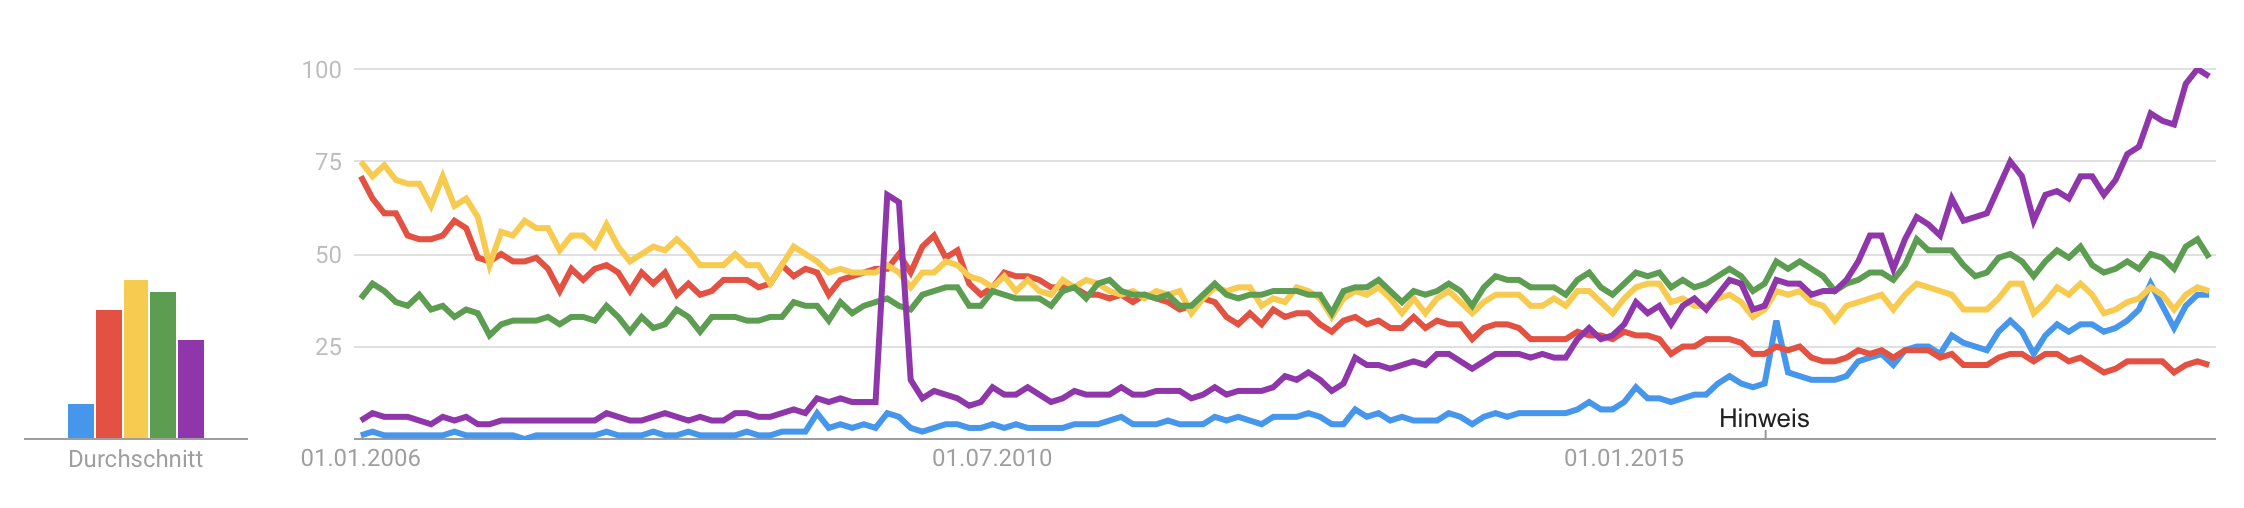
\includegraphics[scale=0.4]{Talk7/img/google_trends}
%  \end{center}
%  \caption{Google Trends for security term between 2006 - 2019}
%  \label{cybersec_google_trends}
%\end{figure}







%\textbf{Length: 2-3 pages}
%\begin{itemize}
%  \item Definition of Cybersecurity (\cite{Bishop2003} and \cite{Bishop2004})
%  \item Description of the history of cyber security (\cite{Hansen2016} and \cite{Bishop2004})
%  \item Information security vs. Cyber security (\cite{VonSolms2013})
%  \item Authentication and Authorization (\cite{Bishop2004} and \cite{Pfleeger2014})
%  \item Cryptography? (\cite{Bishop2004} and \cite{Pfleeger2014})
%  \item Cost-Benefit Analysis, Risk Analysis (\cite{Bishop2004})
%  \item Attack possibilities (Worms, Viruses, Trojan Horses, Bugs, Botnets) (\cite{Bishop2004} and \cite{Pfleeger2014})
%\end{itemize}

\subsection{Blockchain}
\label{subsec:02_blockchain}

Connected to the growing popularity of the Bitcoin Cryptocurrency that conquered the markets of the world, the interest for its underlying technology - the Blockchain - grew in a similar fashion. The idea of having a fully decentralized, tamper-proofed distributed online ledger, fascinated not only the digital world but also other non-digital areas. And while Bitcoin gained a bad reputation due to its fluctuation \cite{Shackelford2016}, the Blockchain, continued its triumphal procession up to a point where one might ask himself: Is the Blockchain a solution for existing problems or is the Blockchain the problem itself? \cite{Stinchcombe2017} \cite{Nielsen2018} \cite{Lunn2015}

In the following subsections, the Blockchain technology is going to be shortly explained and discussed. It is not the goal of this section to give full technical insights into the various mechanisms but to provide a good base of knowledge for the chapters to come.

\subsubsection{The Blockchain in Detail}
The Blockchain is a shared, publicly available online ledger containing a chain of interlinked blocks, that themselves contain transactions between users. \cite{Wust2017}. No single user controls, updates or maintains the blockchain. Instead, every action performed on the blockchain is enforced a consensus amongst all users (nodes) \cite{Shackelford2016}. Because of the way its blocks are interlinked by a cryptographic hash, no changes can be made in the blockchain in hindsight without being traceable.

The Blockchain is, therefore, a data structure that allows humans and computers to interact with each other, without having to rely upon trusted third parties. Instead, it is the controlling power of the data structure itself or put differently, the consensus amongst all users, that assures each parties compliance with their part of a deal. As a result, it allows "people who have no particular confidence in each other [to] collaborate without having to go through a neutral central authority" and becomes "a machine that creates trust" (\cite{Economist2015} as cited in \cite{Shackelford2016}).
\subsubsection{Properties of the Blockchain}
In the following list, the most important properties are compiled \cite{Wust2017}.\begin{itemize}
  \item \textbf{Public verifiability}: The Blockchain has the significant advantage over other data structures that every observer can at all times verify that it is in a valid state and that all the changes made to its blocks are according to the protocol.
  \item \textbf{Transparency \& Privacy}: Everyone with access to it can view the Blockchains transactions over time. However, the more transparent the data is, the less private it becomes.
  \item \textbf{Redundancy}: The Blockchain reduces the chances of losing data by its distributed nature itself. Each peer contains parts of the whole Blockchain locally. The chance that data gets lost is therefore extremely small.
  \item \textbf{Anonymity}: The blockchain per se doesn't know users or real people. Instead, it uses a public-private key-pair that binds every transaction to a specific public key. Committing changes on the blockchain, therefore, leaves no link at all between a real person and his public key.
\end{itemize}

\subsubsection{Common scenarios for usage}
Due to the blockchains various properties, multiple use-cases emerged. Even though the below list is neither exhaustive nor its items disjunct, it shows the most common scenarios for the use of the Blockchain\cite{Wust2017} that are not further discussed in this paper:
\begin{itemize}
  \item Crypto Currencies: From the moment, when the paper by Satoshi Nakamoto (\cite{Nakamoto2009}) was published Blockchains and Crypto Currencies were interlinked. Because a Crypto Currency is per definition a digital asset, the Blockchain suites this use case particularly well.
  \item Supply Chain Management (SCM): In Supply Chain Management the flow of goods includes "various intermediate storage and production cycles" \cite{Wust2017} and the Blockchain is a good way to store and monitor all processes in a tamperproof manner.
  \item Payment and Money Transactions: Transactions between different banks and result in temporary debts between them. This issue can be solved using \textit{Distributed Ledger Technologies}, that make use of a Blockchain to settle debts. 
  \item Decentralized Autonomous Organizations (DAO): "A DAO is an organization that is run autonomously through a set of smart contracts" \cite{Wust2017}. A DAO is therefore fundamentally dependent on the Blockchain, as it relies on decentralized governance of funds enforced by smart contracts.
  \item Proof of Ownership: The idea of proofing intellectual property is one of the most straightforward use cases for the Blockchain. In this scenario, the user registers his or her property (e.g., image, text or another object like land) through the use of an identity function in the Blockchain. "While this does not fully prove ownership, it does provide evidence of ownership if no one else can show that the object was previously published" \cite{Wust2017}.   
\end{itemize}
The excluded use-cases \textbf{IoT}, \textbf{Smart Contracts} and \textbf{E-Voting} can be found under \ref{subsec:03_IoT}, \ref{subsec:02_smart_contracts} and \ref{subsec:03_applications_evoting}.

\subsubsection{The Blockchain and Cybersecurity}
In most cases, the Blockchain technology is used within applications of any sorts and kinds to make them more secure. More secure databases, transaction systems for banks, the replacement of certificate authorities or the security of critical physical infrastructures fall into this category. Another field of applications uses the blockchain directly to mitigate cyber attacks. Examples, therefore, are the mitigation of DDoS Attacks or the handling of PKI related cyber threats. Applications that fall into the second category use the Blockchain more direct and immediate, while the first category uses them on a higher level, to help to reduce the cybersecurity threats in the set up of the application itself. In this paper, both of those categories are covered.
\subsection{Smart Contracts}
\label{subsec:02_smart_contracts}

This section looks at the concept of smart contracts on the example of Ethereum.
Ethereum is a Blockchain ''with built-in programming language'', or in other words a ''consensus-based globally executed virtual machine''.
The Ethereum project started in 2015 and has gained popularity since then. It is second place in terms of market capitalization according to coinmarketcap.com, right after Bitcoin and Ripple \cite{coinmarketcap}.

Nodes in the Ethereum network make up the Ethereum Virtual Machine (EVM). Smart contracts are written in the programming language solidity. They get compiled to bytecode that the EVM can understand.
Once deployed on the Blockchain, the code cannot be changed. Deploying smart contracts means mining them into the Blockchain, thus deploying smart contracts costs a fee like every other transaction. Once they are there, they are part of the Blockchain history. Every smart contract on the Blockchain lives at an address where the contracts exposed functions and variables can interact with. Smart contracts can inherit from smart contracts and can interact with other smart contracts.

Users are able to transfer cryptocurrencies (\textit{e.g.} Ether) to smart contracts.However, sending Ether to a smart contract that does not provide functionality to retrieve those ethers means they are lost forever in the contract. This is crucial especially when designing contracts that implement business logic or any contracts for that matter. Smart contracts should be reviewed and audited carefully and tested for vulnerabilities else its weaknesses can be exploited like in the infamous ``DAO`` attack~\cite{DoaAttack}.

Every transaction on the Ethereum Blockchain costs a fee called gas. Gas is expressed in Ether. The miner that mines a transaction collects the gas associated with it, thus gas serves as an incentive for miners to mine and contribute to the network. There is a defined set of operations with their respective gas costs in the Ethereum yellow paper \cite{ethereumyellowpaer}.
Figure \ref{fig:smart_contract_fees} depicts an excerpt of those costs.

\begin{figure}[ht!]
  \begin{center}
    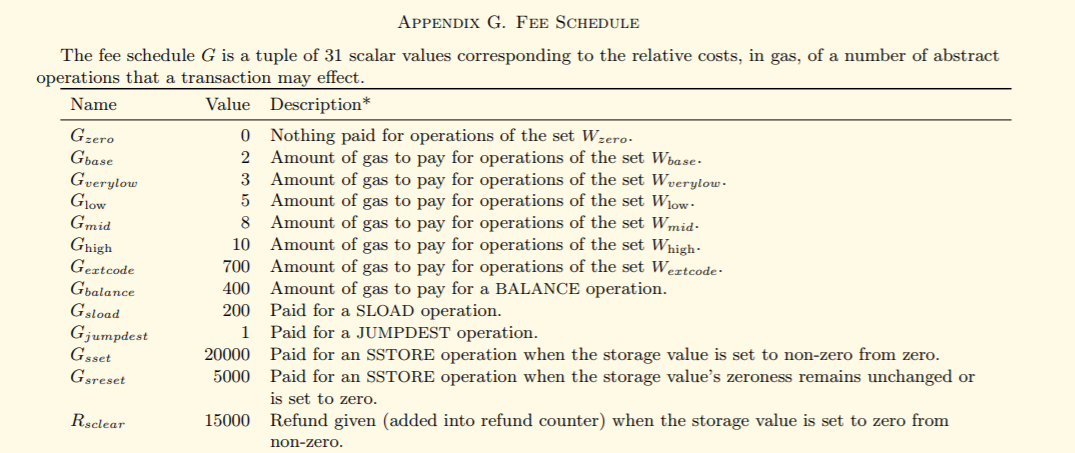
\includegraphics[scale=0.6]{Talk7/img/smart_contracts/gas-fees}
  \end{center}
  \caption{Smart contract fees as shown in the Ethereum yellow paper}
  \label{fig:smart_contract_fees}
\end{figure}

Miners generally prioritize transactions with a higher potential gain (gas). The total gas fee to be paid is calculated by the gas price times the amount of gas to use. If the gas price for a transaction is set high, the transaction is mined to the Blockchain faster. If on the other hand the price is set low, miners choose to mine other transactions first before mining transactions with a lower price. How high the gas price is is determined by the market. During peak network traffic, gas prices are high because as more people want their transaction to go through. Contrarily, prices drop when the network is less utilized.

A transaction has a gas limit that can be set. This is to indicate the maximum amount of gas a transaction can use up before it is aborted. The gas limit times the gas price is the maximum amount the issuer is willing to pay for a transaction. In case of an endless loop, the execution will only last until the gas limit is used up.
If the gas limit is too little, the computation will run out of gas before it is finished, it will be reverted, and the gas paid will be lost. If the gas limit is higher than the amount of gas used, the remaining gas will be refunded to the sender of the transaction.

Miners can only include so many transactions in a block that block gas limit is not exceeded. This is also not a fixed value as miners can vote with each block to increase or decrease the block gas limit by a certain amount. Block gas limit serves to keep propagation of blocks and transaction time low by essentially limiting the size of the blocks.

The following overview sums up the key terms as mentioned above \cite{blockgeeks}:
\begin{itemize}
  \item {\textbf{gas}: How much gas a transaction needs }
  \item {\textbf{gas prize}: How much Ether a unit of gas costs, determined by the market}
  \item {\textbf{gas limit}: Maximum amount of gas to use up for a transaction}
  \item {\textbf{transaction fee}: Gas used times gas price}
  \item {\textbf{block gas limit}: Maximum sum of gas of all transactions in a block}

\end{itemize}

In fact, not all smart contract interactions cost gas. Functions that do not modify the state of a contract, and hence the Blockchain, do not need to be mined by a miner.
Calling those functions will still use gas, because every operation in the EVM uses gas, but that gas is refunded immediately as calling those functions does not result in a transaction.
In solidity those functions have the modifier ``pure'' or ``view''. Functions denoted with ``pure'' do not even read state variables. Both those functions can be run on a single node in the EVM and
nothing has to be propagated to the network. Thus, no transaction has to be mined into the Blockchain and no gas fee has to be paid~\cite{blockgeeks}.

\begin{lstlisting}[language=Solidity,caption={Smart contract example},,label={solidity_example}]
  pragma solidity 0.5.0;

  contract MyContract {

    string private myString = "foo";

    function getString() view returns (string) {
        return myString;
    }

    function setString (string _string) {
        myString = _string;
    }
  }
  \end{lstlisting}

In the smart contract example, presented in Listing~\ref{solidity_example}, the functions ``setString'' modifies the state, namely the variable ``myString'', thus a transaction needs to be recorded in the Blockchain and gas has to be paid.
The function ``getString'' on the other hand is denoted with the keyword ``view'', no state variables are modified so no transactions are required and no gas fee has to be paid.

Smart contracts allow programming on the Blockchain which opens up a multitude of possibilities also in the context of cyber security for which upcoming sections discuss some solutions.



\newpage
\section{Blockchain Application in Cybersecurity}
\label{sec:03_related_work}

Having built the theoretical foundation in section \ref{sec:02_background}, we now focus on the main research question of this work and summarize recent research in the intersection of blockchain and cybersecurity. The subsequent sections can broadly be separated into a low-level, more technical part (sections \ref{subsec:03_ddos} and \ref{subsec:03_pki}), and a high-level, more application-oriented part (sections \ref{subsec:03_IoT} and \ref{subsec:03_applications}).

Section \ref{subsec:03_ddos} first presents some of the possible blockchain-based solutions that have been developed as a countermeasure to DDoS attacks, alongside a comparison to currently existing countermeasures and the potential motivations for attackers in a DDoS context. Subsequently, section \ref{subsec:03_pki} goes into the potential application of blockchain to rebuild a key part of the internet security infrastructure, specifically the current idea of PKI's. On a higher level, section \ref{subsec:03_IoT} then presents some of the critical issues in securing IoT devices, as well as how they could be approached with blockchain technologies. Finally, \ref{subsec:03_applications} summarizes the currently productive applications of the blockchain in a broad cybersecurity context, as well as some other application areas that are still part of current research.

\subsection{Distributed Denial of Service (DDoS)}
\label{subsec:03_ddos}

% TODO add an army of zombies

% Introduction describing the base of such attacks
A Distributed Denial of Service (DDoS) attack has become a popular way to cripple servers of an institution or a private person. How is it possible for attackers to execute such attacks? The current internet design has the purpose of moving packets from a source to a known destination. The network itself forwards all packages at minimal cost and generally outsources the complexity, including security, transport reliability and quality of service to the sender and receiver of the transported packages. This concept has been called the \textbf{end-to-end paradigm}. As no intermediary entity will step in, a party (either sender or receiver) can damage its opposition by using attack possibilities such as IP Spoofing or the aforementioned DDoS attacks \cite{Mirkovic2004}. By faking the source address in the header of a packet, the sender can hide its identity. This security issue is called IP Spoofing \cite{Cloudflare2019}. As described in \cite{Mirkovic2004}, the following security issues raise opportunities of attacks:

\begin{itemize}
  \item \textbf{Limited internet resources}: Every host or service has hardware limitations that users may consume.
  \item \textbf{Highly interdependent internet security}: No matter how secure a host may be configured, DDoS attacks always depend on the security of others within the Internet.
  \item \textbf{No collocation of intelligence and resources}: The intermediate network has plentiful resources, as they forward packages at minimal costs.  In contrast, the end networks only invest in as much bandwidth as they planned to use for their services.
  \item \textbf{No enforcement of accountability}: As described above, attackers can escape from accountability by using IP Spoofing mechanisms.
  \item \textbf{Distribution of control}: In a world of a distributed network, such as the Internet, multiple clients participate in the network. Each one of them has different security mechanisms. No global control entity can define a security policy or standard.
\end{itemize}
% Additional reasons/base of attacks
Since the number of connected devices has increased due to IoT devices such as connected cameras, or smart fridges, attackers have a growing capacity to take control of unsecured devices \cite{Rodrigues2017}. By operating multiple such attacking entities called computer bots (clients that have been taken over by malware) remotely, attackers try to overflood a website, a network or a server and prevent rightful users from accessing the application. The service is either responding slowly or shut down entirely. More precisely, attackers send a stream of packets to the victims, which consume all capacity of hardware resources and therefore make it unavailable for legitimate clients to access the service provider.

Another popular way for an attacker is to send malformed packets to negatively impact the availability of the application service. Those packets confuse the web application or some protocols on the victims' hardware and force the server to reboot. There are probably additional possibilities to attack services on the internet. Such attack possibilities are mostly discovered first once they have been exploited in a significant attack and servers have been down for a particular time \cite{Mirkovic2004}.

% DDoS procedure
The procedure of a DDoS attack is split into the following phases: An attacker recruits multiple agents (clients) into which the attacker injects malicious code. Attackers often hide the identity of infected clients by using IP Spoofing mechanisms \cite{Mirkovic2004}.

% TODO Difference DoS and DDoS?

% Motivation behind DDoS
Multiple incentives exist to attack clients using DDoS attacks. Unfortunately, the primary goal of such an attack is to damage the selected victim. Motives may be found in prestige (gaining respect within the hacker community when attacking popular websites or services), personal hatred, material gain (damaging competitors by attacking them), any political reasons, or blackmailing others \cite{Mansfield-Devine2015, Mirkovic2004}.

%  Generalize possibilities of current mitigation strategies
Various companies currently offer DDoS protection services, such as Cloudflare or Akamai, and their number is increasing \cite{Pras2016}. Those solutions serve as a proxy and manage routing, load balance, and drop traffic when a DDoS attack occurs. For all solutions, a third party DDoS Protection Service (DPS) provider is required, resulting in extra cost, as the analyses are performed in the cloud \cite{Rodrigues2017}. Those cloud-based defense services could become a communication bottleneck because the traffic (download and processing) is dependent on a single provider. By utilizing resources from other companies, the workload of mitigating DDoS attacks can be shared \cite{Rodrigues2017}.

% TODO More about DOTS (DDoS Open Threat Signaling) an IETF proposal
% TODO probably explain Gladius?
The Internet Engineering Task Force (IETF) additionally is proposing a protocol called DDos Open Threat Signaling (DOTS) that requires both clients and servers. A new protocol is required which has to be maintained. DOTS clients have to register to a DOTS server and use this protocol among the agents to organize the DDoS protection \cite{Rodrigues2017}. In the following sections, various approaches to mitigating DDoS attacks without the need to deploy a new protocol are illustrated.

\subsubsection{DDos Mitigation with Smart Contracts}
% \cite{Rodrigues2017}
This concept investigates a possibility to mitigate a DDoS attack in a fully decentralized manner using smart contracts and their underlying blockchain. These technologies allow sharing information (detection and mitigation mechanisms as well as IP addresses) about attacks in an automated and decentralized system \cite{Rodrigues2017}.

As described in \ref{subsec:02_smart_contracts}, a smart contract is a software that is made to help contracts being able to execute and verify on their own. To do so, there has to be an infrastructure that implements, verifies and enforces the negotiation of those smart contracts by using particular computer protocols and that runs fully decentralized. As known from \ref{subsec:02_Blockchain}, a blockchain ensures permanent storage and provides obstacles to manipulation of content and is thus an ideal infrastructure for smart contracts. Nodes participating in the blockchain run a smart contract by executing and validating a script and thereafter storing the contract and the results in a new block \cite{Rodrigues2017}.

% Proposed System Architecture
As presented in \ref{system_architecture} the architecture is composed of three components. The customers report IP addresses to the blockchain via smart contracts. The autonomous systems (AS) retrieve lists containing these addresses and implement DDoS mitigation techniques. All participants interact with the underlying blockchain \cite{Rodrigues2017}.

The web server of one autonomous system (AS) is a victim of a DDoS attack. Participants that have proven ownership of their IP then create a smart contract that stores all IP addresses of attackers. Subscribed systems receive updated lists of IP addresses every 14 seconds, as the underlying blockchain, Ethereum, creates new blocks within that timeframe. As soon as all other autonomous systems receive the list of attackers, various mitigation strategies may be triggered tailored to the specific domain \cite{Rodrigues2017}.
\begin{figure}[ht]
  \begin{center}
    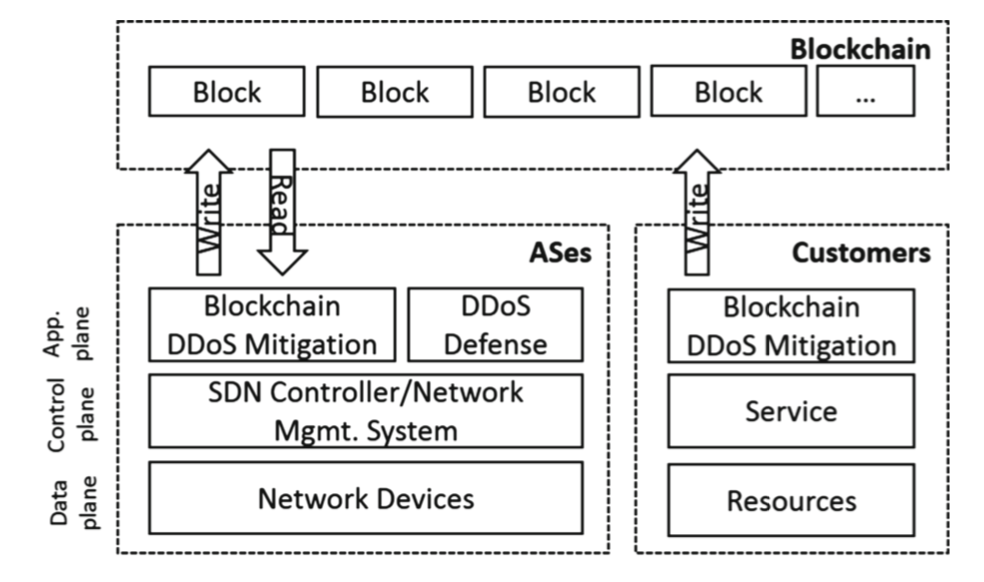
\includegraphics[scale=0.6]{Talk7/img/ddos/collaborative_ddos_mitigation_system_architecture}
  \end{center}
  \caption{System Architecture}
  \label{system_architecture}
\end{figure}

% Conclusion
This approach uses an already existing and publicly available distributed infrastructure to adumbrate IP addresses that are either white- or blacklisted. This approach serves well as an additional security mechanism to existing DDoS defense systems across multiple domains by using an Ethereum blockchain without transferring the control of their internal network to a third party. For large-scale attacks, this approach currently is not supported well, but this issue will be addressed in future work \cite{Rodrigues2017}.


\subsubsection{Mitigation-as-a-service in cooperative network defenses}
% \cite{Mannhart2018}

% Short introduction
With cooperation between multiple domains, various collaborating autonomous systems (AS) can alleviate DDoS attacks by redirecting excessive traffic to other domains that filter the traffic. Incentives ensure the use of mitigation-as-a-service for cooperative network defenses. By paying fees, enterprises or individuals can subscribe to such a cooperative defense network and protect themselves from future attacks \cite{Mannhart2018}.

As soon as a target detects an attack, it sends a request to all participating autonomous systems to mitigate the current attack. Subsequently, a mitigator that is responsible for the range being attacked then either accepts or declines the mitigation request. By using a \textbf{proof-of-mitigation}, the completion of the mitigation has to be confirmed, and the target can pay the mitigator. As this proof-of-mitigation has to satisfy time constraints, tamper-evidence, and reproducibility, this proof has to be executed automatically during the current time window. Additionally, any user interaction has to be excluded to ensure efficiency \cite{Mannhart2018}. Various approaches creating such proof will be described and discussed in this section and have been tested on different metrics related to security and practicability.

\paragraph{Marketplace of Mitigation VNFs}
Virtualized  Network Functions (VNF) can be deployed on any hardware without additional configurations. The concept of Network Function Virtualization (NFV) can, therefore, provide an efficient solution by virtualizing a single function in the network as seen in \ref{ddos_marketplace_vnf}. All autonomous systems involved in the cooperative network could load the VNF image directly from the marketplace, which then provides the mitigation service hosted on virtual devices. By comparing the hashed checksum of the VNF image to a known value from the marketplace, the integrity of the VNF image will be checked. Additionally, local caching of all VNFs avoids large load on the marketplace. A big advantage of this approach is the high degree of isolation, as the VNFs consist of the minimal code necessary to handle the mitigation. Unfortunately, the target still needs to trust that the mitigator only runs untampered VNFs directly from the marketplace \cite{Mannhart2018}.
\begin{figure}[ht]
  \begin{center}
    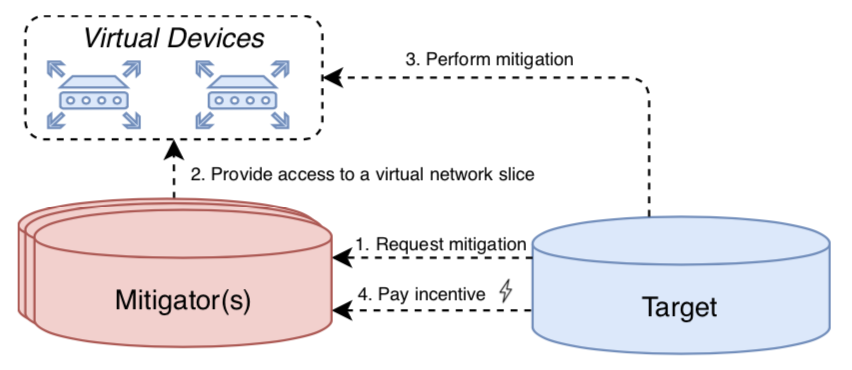
\includegraphics[scale=0.5]{Talk7/img/ddos/cooperative_network_marketplace_vnfs}
  \end{center}
  \caption{Marketplace of Mitigation VNFs}
  \label{ddos_marketplace_vnf}
\end{figure}

\paragraph{Trusted Computing}
In contrast to the previous approach as illustrated in \ref{ddos_marketplace_vnf}, the mitigator directly initiates the mitigation. So-called Trusted Platform Modules (TPM) enable secure storage of hashes. This allows that only the code that is approved by the cooperative defense will be run on the system. VNFs create a defense network where trusted and known VNFs always handle requests for mitigation without trusting the responsible operator that provides the mitigation service to the autonomous system.  A big disadvantage of trusted computing is the strict hardware requirement, as the TPM is only available as a standalone chip or integrated into the motherboard \cite{Mannhart2018}.

\paragraph{Secure logging}
As mitigators can use full network infrastructure, they are allowed to proof the mitigation using the available traffic data. By having a detailed log of network activities, they could prove the successful mitigation by identifying a reduction in the traffic from the attack source to the DDoS target. A mitigation-proof based on the log files decreases the complexity of the proof. The aforementioned log file has been created on an isolated system (which requires no additional trust) and therefore has to be checked about its integrity by a third party. A disadvantage comes with high-volume attacks which create large log files. These large files introduce additional delays as the log files have to be transferred for remote auditing \cite{Mannhart2018}.
\begin{figure}[ht]
  \begin{center}
    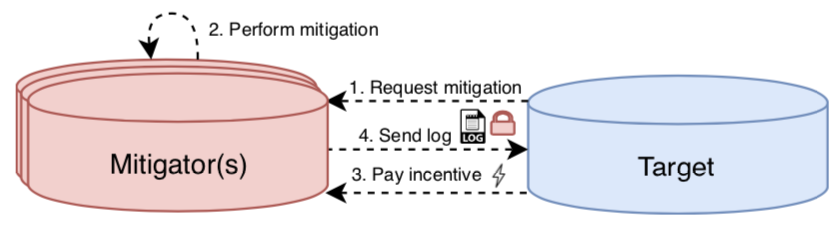
\includegraphics[scale=0.5]{Talk7/img/ddos/cooperative_network_secure_logging}
  \end{center}
  \caption{Secure logging}
  \label{ddos_secure_logging}
\end{figure}

\paragraph{Network Slicing}
Since network virtualization technologies and Software-Defined Networks (SDN) have advanced in recent times, they both serve as a basis for network slicing as a service. When the attack target requests mitigation services, it gains access to the virtualized network slice of the mitigators autonomous system. The slice is then configured to provide access for all attacking IP addresses that have been requested within the mitigation request \cite{Mannhart2018}.
\begin{figure}[ht]
  \begin{center}
    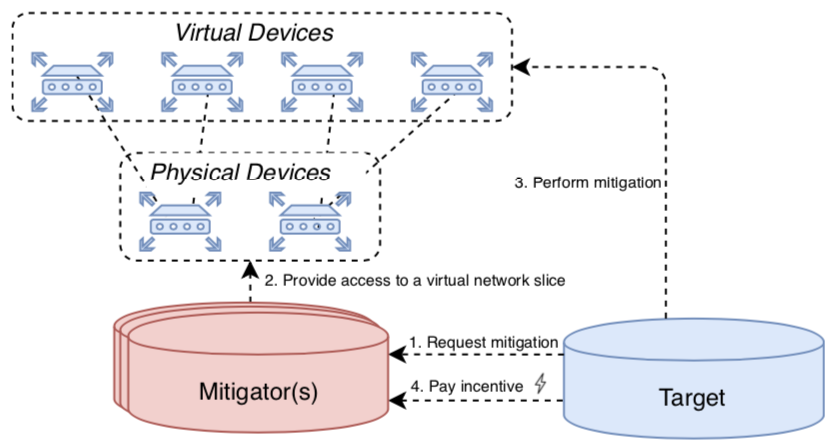
\includegraphics[scale=0.5]{Talk7/img/ddos/cooperative_network_network_slicing}
  \end{center}
  \caption{Network Slicing}
  \label{ddos_network_slicing}
\end{figure}

As a final consideration, the authors remarked that none of the preceding methods could on its own be used to address a trade-off between practicability and security when qualitatively comparing all four approaches. However, combining some of these methods could lead to a practical as well as secure solution \cite{Mannhart2018}.

\subsubsection{Multi domain DDoS Mitigation based on blockchains}
% \cite{Rodrigues2017a}
Another approach repeatedly uses smart contracts as a means of advertising information across multiple domains. The architecture as seen in figure \ref{ddos_multi_domain_architecture} involves the following entities: \textbf{Software-Defined Networks (SDN)} facilitate the development of customizable security management; \textbf{Network Function Virtualization (NFV)} that are provisioned in generic hardware strengthen security policies through virtualized functions; an Ethereum-based \textbf{blockchain} is a base for all participants of the cooperative network to advertise DDoS attacks within a timeframe of 14s, in which a new block is mined; and a \textbf{smart contract} that stores black or whitelisted IP addresses of customers \cite{Rodrigues2017}.

\begin{figure}[ht]
  \begin{center}
    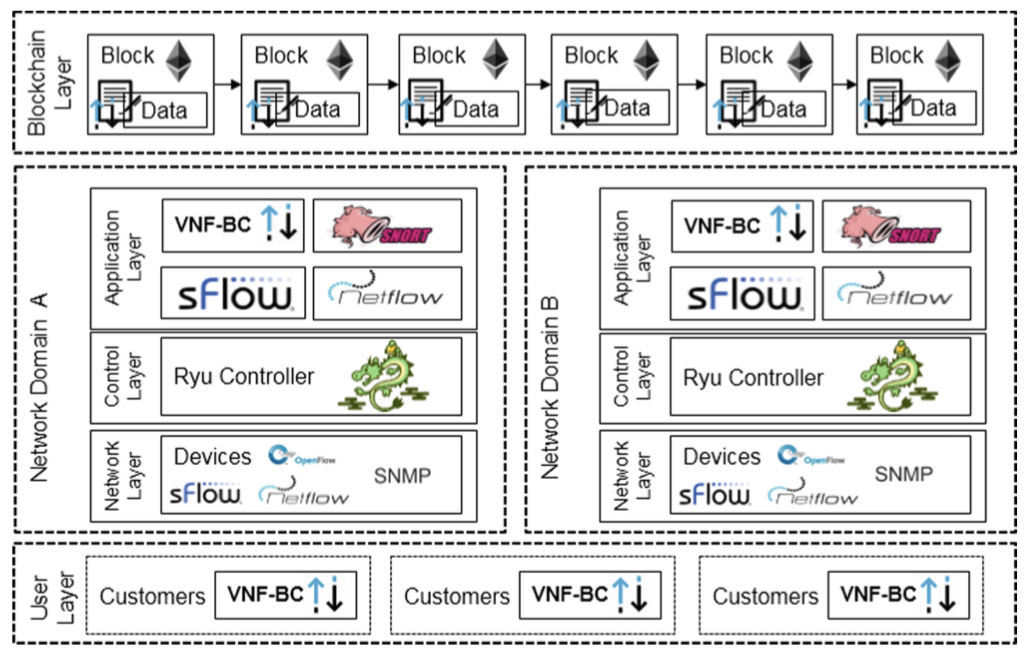
\includegraphics[scale=0.5]{Talk7/img/ddos/multi_domain}
  \end{center}
  \caption{Multi-domain architecture}
  \label{ddos_multi_domain_architecture}
\end{figure}

%  conclusion of paper
This architecture is based on key technologies such as software-defined networks (SDN) and network function virtualization (NFV). Blockchain and smart contracts advertise DDoS attack information to broadcast white or blacklisted addresses without building any distribution mechanisms or protocols \cite{Rodrigues2017}.

\subsubsection{Blockchain Signaling System (BloSS)}
% https://github.com/blockchain-signaling-system/bloss-core
% https://github.com/savf/BloSS
% \cite{Rodrigues2019}

Similarly to \cite{Rodrigues2017}, this approach deals with cooperative, multi-domain DDoS defense systems, but it presents a Blockchain Signaling System (BloSS) which is a somewhat technical approach of deploying hardware simplifying signals of DDoS attacks. Principal components for a BloSS are smart contracts that describe how information has to be transferred between Autonomous Systems (AS) and decentralized applications that include parameters defining the interaction of AS. Additionally, a consortium based blockchain, differentiating from the public and private blockchains, serves as an intermediary level of confidence.

An Autonomous System (AS) creates a wallet and notifies a smart contract that stores some information. The smart contract then implements a method to reclaim addresses published by other systems by querying a central smart contract. This central contract is used to configure all involved smart contracts with updated information on their managed IP networks, as the addresses of the involved wallets are immutable. In order to prevent free-riding peers (parties that only consume without any contribution), an incentive mechanism needs to be set by defining tokens \cite{Rodrigues2019}.  % TODO what do they do?

%  TODO more about Architecture and Hardware?

\subsection{Public Key Infrastructure (PKI)}
\label{subsec:03_pki}

Public Key Cryptography serves as one of the cornerstones of modern communication systems and technologies, also including the Blockchain. Entities can secure their communication asynchronously using a pair of keys (public and private). After the distribution of its public key, an entity can be contacted by anyone via securely encrypted channels.

What makes this type of cryptography so convenient is that its security does not depend on any shared hidden secret (\textit{e.g.}, a passphrase). An entity encrypts its message using the public key of its counterparty, after which only the supposed recipient can decrypt the message with its private key. While the public key and private key always belong to the same communication channel, it is practically not possible to infer the private key from the public key. This means that the public key can be distributed without considerations about the trustworthiness of potential recipients (\textit{e.g.}, publicly on online platforms) \cite{straub_tobias_usability_2006}.

For a private exchange between two to a few counterparties, the simple approach of distributing public keys out-of-band (\textit{e.g.}, in person) might suffice to establish sufficient confidence and trust. As soon as we consider communication networks on a larger scale, an in-person exchange between all parties in the network would no longer be feasible. In such a case, one or more trusted, often centralized entities need to support the process of establishing trust \cite{straub_tobias_usability_2006}.

PKI is the summary term for an infrastructure that enables secure communication through such trusted entities. As described in \cite{straub_tobias_usability_2006}, a PKI "lets participants communicate with each other securely using public key cryptography and allows them to verify each other's keys with the help of certificates and trust relations."


\subsubsection{Existing PKI Systems}

Traditional PKI systems are most visibly used for communication over the web. Before two entities (\textit{e.g.}, a server and a client) can securely communicate over HTTPS/TLS, the domain name of the server must have been validated and certified by a certificate authority (CA). A CA is an entity that has the authority over issuing certificates for a given PKI namespace (\textit{e.g.}, domain names or a subset thereof).

A PKI certificate verifies that the given name-value (\textit{e.g.}, domain name and public key) binding is authentic and is itself signed with the key of a CA. The trustworthiness of a CA is signed by a higher-level CA, building a chain up to a root-level CA that ultimately needs to be trusted without verification. When establishing communication with a server over HTTPS, a client verifies the identity of the server according to its certificate, and client and server confidentially decide on a data encryption secret by employing asymmetric encryption. All further message and data exchanges are secured with symmetric encryption \cite{straub_tobias_usability_2006}. The procedures of PKI management as employed in HTTPS/TLS, as well as many other systems and private infrastructures, are standardized by the IETF in the X.509 standard \cite{adams_internet_2015}.

Contrary to the centralized approach, the Pretty Good Privacy (PGP) architecture is based on a decentralized web-of-trust where all participants manually define their trust anchors (\textit{i.e.}, which entities to trust as the anchor for a certificate chain) instead of relying on a predefined trust store as included in operating systems or browsers \cite{straub_tobias_usability_2006}. While PGP is in relatively broad use for secured email communication, this work focuses mainly on centralized infrastructures for their approachability with Blockchain architectures.


\subsubsection{Threat Model for Public Key Infrastructures}
\label{subsubsec:threat_model_pki}

PKI systems allow for an establishment of trust and a secure exchange between parties that do not necessarily know each other. However, both participating parties need to trust the centralized CA to issue valid certificates. The most visible threat to a PKI system is, therefore, an attack on this centralized trusted party.

Any such kind of attack could, if successful, allow an intruder to generate fraudulent certificates, which could then be used to impersonate one or more of the parties and perform a proxied man-in-the-middle attack. In such an attack, the attacker acts as a proxy that intercepts messages between the parties, decrypts and extracts their contents, and redirects them to the original recipient, making it very difficult for the participants to figure out they are being intercepted \cite{zusman_criminal_2008}.

In the concrete example of a web certification authority, domains are most often validated by merely sending an email to an address on the domain to be certified (\textit{e.g.}, webmaster@xyz) or by verification of DNS records. This indirect verification creates vulnerabilities on several levels, as emails and DNS settings are managed by separate entities that could be attacked. CAs have also been known to issue fraudulent certificates on government request (\textit{e.g.}, for censorship), or through simple human error \cite{zusman_criminal_2008, zohar_blockchain-based_2019}.

As centralization in PKI systems leads to a big attack surface, developing approaches that can function without the need for any such central entities (\textit{e.g.}, CAs) have been a topic of several publications in recent years. The following sections provide a more detailed overview of decentralized PKI in general as well as more specific applications in the area of web certification. While there are many other types of attacks on PKI (\textit{e.g.}, obtaining a private key through social engineering or directly attacking the encryption protocols), we focus on the critical aspect of centralization in this work.


\subsubsection{Decentralized Public Key Infrastructures}

\paragraph{Namecoin}

A foundational work that introduced the idea of applying Blockchain to the decentralization of naming systems was initially created to rebuild the Domain Name System (DNS) such that it can work without centralized DNS servers. Much like central PKI entities, DNS servers can be exploited and, if hacked, can be a threat to large parts of the internet user base.

The main idea of Namecoin is to store all DNS-related naming information in a Blockchain ledger that enforces state updates to occur via appended transactions. All entities in the network share a copy of this ledger and can independently lookup the records associated with a name. Records are owned, and can only be modified, by a given cryptographic identity \cite{noauthor_namecoin_nodate, ali_blockstack:_2016}.

While this approach to naming provides the benefit of decentralization, it comes with challenges regarding security, performance, and scalability. The Namecoin Blockchain is a fork of the Bitcoin Blockchain and shares most of its technicalities and limitations but progresses a separate ledger. This means that it has a separate and much smaller set of miners, making it very vulnerable to 51\% attacks (where an attacker controls a majority part of the computing power and can rewrite the chain) or DDoS. Even though Namecoin implements merged-mining (\textit{i.e.}, it allows bitcoin miners to participate in Namecoin mining), its computation is mainly concentrated on one big pool of miners with >50\% of the computational power \cite{noauthor_namecoin_nodate, ali_blockstack:_2016}.

In addition to the limitations on a security level, Namecoin also struggles with regards to performance (\textit{e.g.}, transactions per second). As the block size in bitcoin and its forks (\textit{i.e.}, Namecoin) is relatively small, there is a limited amount of data that can be stored in transactions and processed in a block, which severely limits the throughput of transactions and can lead to issues in a DNS use case.

\paragraph{Blockstack}

The Blockstack system was initially based on the Namecoin Blockchain using a dedicated namespace. Using the initial system called Blockstack ID, users could link their username with their public key, as well as some additional data. To work around the issues of limited storage within a block, Blockstack ID would connect related key-value pairs using a linked list data structure mapped to the Blockchain \cite{ali_blockstack:_2016}.

Mainly due to the security implications of Namecoin also applying to Blockstack ID, its maintainers have intermittently developed a new approach that replaces Namecoin with the Bitcoin Blockchain. Contrary to its predecessor, Blockstack does not store its data directly in the Blockchain. Instead, the Blockchain only stores hashes of the data, while the data itself is stored in external systems \cite{ali_blockstack:_2016}.

The Blockstack architecture introduces a novel approach that is called the virtualchain. The virtualchain is a logical structure built on top of a Blockchain that processes transactions relevant to the Blockstack system and implements a state-machine over these transactions. When state updates occur, new transactions are encoded and written to the underlying Blockchain (subject to consensus). The virtualchain is used to compute a global state of who owns what names and what is associated with these names. These components form the control plane of the Blockstack architecture \cite{ali_blockstack:_2016}.

Instead of storing the production data in Blockchain productions, Blockstack only appends hashes and pointers to the real data to the Blockchain. The production data is managed by a separate data plane that consists of routing as well as actual persistence capabilities. Similar to the approach taken by traditional DNS, the routing layer is based on zone files that contain all routes/records for any given name. The actual persistence layer then stores whatever data is to be associated with a record in a database or another storage system \cite{ali_blockstack:_2016}.

Separating the architecture into a control and data plane allows for efficient lookups of data against the data plane, while still allowing for verification of the data stored therein using the control plane. As a hash of the zone file is stored alongside its name in the Blockchain, a low-level transaction with consensus is necessary to modify the zone file that is associated with a name. Furthermore, if hashes of record contents are put inside the zone file, these contents also become immutable without consensus \cite{ali_blockstack:_2016}.

The Blockstack system architecture also offers possible solutions for several fundamental problems regarding the storage of associated data. The production data is stored outside of the Blockchain, which works around the limited amount of storage per block. Additionally, the data that needs to be replicated across participants in the network is limited, as transactions only contain hashed and encoded information \cite{ali_blockstack:_2016}.

\paragraph{Bitforest}

Approaches like Blockstack are possible solutions for the deployment of a fully decentralized PKI system that cannot be controlled or censored by any one entity. However, while this might be advantageous for some cases, organizations that deploy a PKI, even if it is decentralized, more often want to keep some control over their namespace. Without any such means of control, PKI systems are vulnerable to many kinds of abuse. An exemplary kind of abuse is called name squatting and refers to the preemptive reservation of names under the expectation of future profit (\textit{e.g.}, through auctioning off the name) \cite{dong_bitforest:_2018}.

Similarly to the Blockstack architecture, the approach taken by Bitforest is based on a data structure on top of a Blockchain. However, Bitforest allows an organization to keep control over who participates in their namespaces. A namespace administrator can define mappings of names to indices in a binary search tree, where for each index, a list of all current and preceding values is stored \cite{dong_bitforest:_2018}.

However, even though an administrator defines the mapping, only the owner of the name can update the associated value by appending to the log of the corresponding name. This maintains the critical property of identity retention, meaning that only the owner and no centralized entity can ever change a value that has been associated with a name \cite{dong_bitforest:_2018}.

When clients need to look up the current value that corresponds to a name, they search for the corresponding index in the directory maintained by the namespace administrator. Querying the search tree for the given index yields the current value, while verifying the previous log entries ensures the integrity of the name \cite{dong_bitforest:_2018}.


\subsubsection{Web Certifications using Blockchain Technologies}

One of the most important application areas of PKI systems is the certification of the integrity of domains in the world wide web. Through its exposure to a substantial number of people, the web certification system is one of the most widely exposed and has been subject to several critical vulnerabilities and attacks. Recent research tries to prevent some of these attacks by employing a Blockchain-based web certification infrastructure that does not need to rely on trusted central entities.

\paragraph{Ghazal}

In the traditional web certification model, domains and their owners are validated by trusted certification authorities. The most popular means of validation is domain-validation, meaning that only the association between the public key and domain name is certified. This approach suffers from the many critical issues due to indirections as described in Section \ref{subsubsec:threat_model_pki}.

Ghazal proposes a new uni-authoritative paradigm for web certification and domain infrastructure. Concretely, no single authority should be needed to certify entities or register domains, as the Blockchain itself could serve as a sort of authoritative entity. This approach has the potential to solve many of the vulnerabilities occurring due to indirections and centralization in general \cite{zohar_ghazal:_2019}.

The foundation of the Ghazal prototype is built on a smart contract on the Ethereum Blockchain. The contract specifies all procedures regarding the registration, transfer, and expiration of domains, as well as the associated values and certificates. Upon registration of a domain name in the \textit{.ghazal} namespace, the owner can assign arbitrary values to the name (including public keys/certificates). Registrations and other operations incur a fee that is paid to a block-hole account on the Ethereum network, meaning that nobody can spend the fee again \cite{zohar_ghazal:_2019}.

While a uni-authoritative paradigm could solve some of the issues in today's web certification, browsers and operating systems would need to be extended to support such functionality. For example, to support the current Ghazal proposal, \textit{.ghazal} domains would need to be recognized, processed, and verified differently from the remainder of sites on the web \cite{zohar_ghazal:_2019}.

It is also still a topic of research if and how a decentralized system could support domain lookups efficiently without the need for storing the entire Blockchain on each client device. Furthermore, the approach taken by Ghazal is plagued by new issues that arise through the removal of all central entities. For example, if a domain owner's private key were to be lost, the corresponding name could never be reassigned \cite{zohar_ghazal:_2019}.

\paragraph{Certificate Recovation and Transparency}

Certificate Transparency (CT) is a recent improvement to the traditional web certification model. When CT is enforced by a browser (\textit{e.g.}, modern versions of Chrome), the browser only accepts certificates without warning if they have been published to a public append-only log of certificate issuances. This measure has been introduced to counteract the malicious issuance of certificates by hacked CAs or through compulsion or malfeasance \cite{zohar_blockchain-based_2019}.

While CT in traditional web certification can already improve web security significantly, it is only a reactive measure, meaning that fraud can still occur but are probably recognized more quickly. \cite{zohar_blockchain-based_2019} proposes that certificate issuance as well as handling the revocation of certificates could be moved to a Blockchain-based system, preventing the issuing of malicious certificates entirely without the approval of the domain owner.

In the solution proposed in \cite{zohar_blockchain-based_2019}, certificate authorities would not hold the solemn authority over certification. Instead, a certificate would only ever be valid if the associated web server cooperates in their publication by publishing the CA-issued certificate to a public certificate issuance Blockchain. Browsers would then only accept certificates that have been both issued by a valid CA and published to the Blockchain. By additionally enforcing a short expiration time on certificates, certificates that need to be revoked could just not be renewed, causing the CA to issue a revocation. Similarly to the approach taken in Ghazal, a key challenge of such an approach is that clients need to maintain a copy of the certificate Blockchain to verify the integrity of certificates.


\subsubsection{Keyless Signature Infrastructures and Blockchain}

A Keyless Signature Infrastructure (KSI) is the basis for an alternative approach to verification of the integrity of documents that does not depend on the secrecy of private keys. A document that is submitted to a KSI is first hashed and then added to a Merkle hash-tree containing all documents processed in the same round (\textit{i.e.}, with other documents that arrived around the same time). The signature token received upon document submission can then be used to check whether a document was contained in the tree at the given time. By following the path encoded in the signature token, it must be possible to reconstruct the root-hash of the entire tree \cite{hutchison_keyless_2013, jamthagen_blockchain-based_2016}.

The KSI architecture processes incoming signature requests in rounds (\textit{e.g.}, one round per second) and, after completion of a round, appends the root-hash of the generated hash tree to a global tree (``hash calenda''). The root of this global tree is then periodically published as a trust anchor that can be used to verify the presence of a document at a point before its publication \cite{hutchison_keyless_2013}. Contrary to the approach of signing documents with one's private key, this approach depends on the infrastructure (\textit{i.e.}, signing servers) to sign the document into the tree. This is what makes possible keyless signing but also incurs a dependency on the availability of the KSI to sign a document \cite{jamthagen_blockchain-based_2016}.

The authors of \cite{hutchison_keyless_2013} suggest that the root-hash could be published to broad-reach media like newspapers in monthly iterations. This would allow verification of a document's integrity even without the KSI infrastructure, as one can compute the root-hash and compare it to the one published. However, this approach is inefficient in that it needs manual verification against an external medium and can only be performed with a reasonable publishing frequency \cite{jamthagen_blockchain-based_2016}.

The Blockchain-based approach presented in \cite{jamthagen_blockchain-based_2016} improves the efficiency by publishing to the Blockchain in an increased frequency such that one can more granularly verify when a document was signed (\textit{i.e.}, added to the tree). Additionally, the break between media is no longer necessary, as signatures can be automatically verified based on the Blockchain contents. When publishing to the Blockchain, the frequency can be increased to several times per hour, as it is only limited by the throughput of blocks being mined \cite{jamthagen_blockchain-based_2016}.

\subsection{Internet of Things (IoT)}
\label{subsec:03_IoT}

Figure \ref{fig:iot_market} shows the predicted market impact of IoT in billion U.S. dollars in each category.
Not only is IoT relevant for the Industry 4.0 with smart factories or the move toward smart cities. IoT also
impacts everyday life with smart homes, vehicles and healthcare. This section aims to present collected solutions on how  Blockchain technology can help with security with regards to IoT and its applications.


\begin{figure}[ht!]
  \begin{center}
    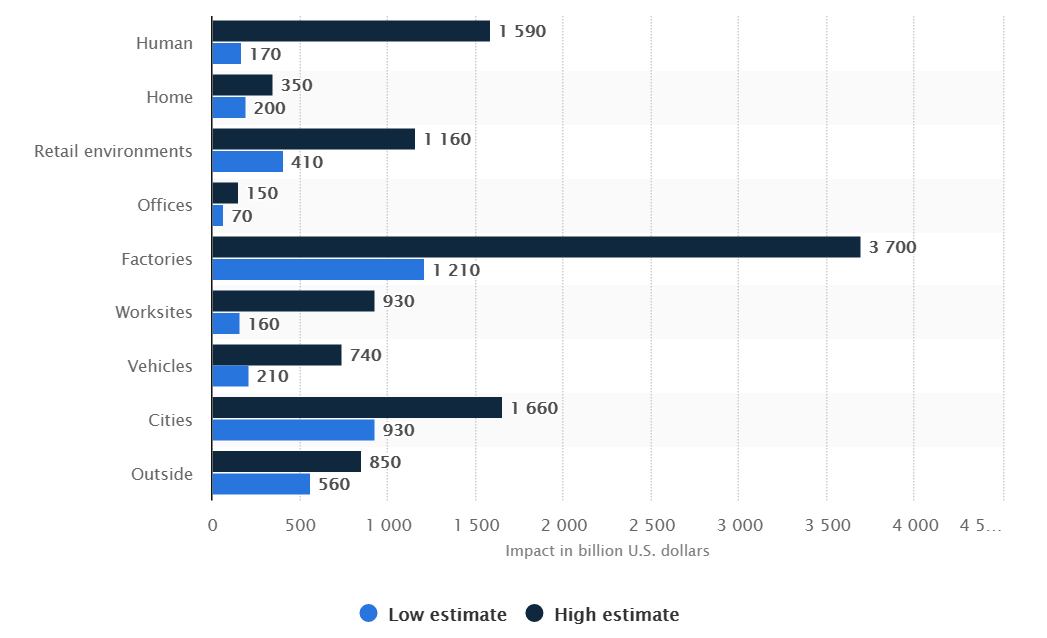
\includegraphics[scale=0.6]{Talk7/img/iot/iot_statista}
  \end{center}
  \caption{Iot market impact, Source: \protect\url{https://www.statista.com/statistics/580778/worldwide-internet-of-things-economic-impact-forecast/}~\cite{StatistaIoT} }
  \label{fig:iot_market}
\end{figure}

Banerjee et. al. in \cite{Banerjee2018} state that given the potentially sensitive nature of IoT datasets,
there is a need to develop a standard for sharing IoT datasets among the research and practitioner communities
and other relevant stakeholders. They propose two examples to use Blockchain for IoT security. One for IoT dataset sharing using Blockchain and another one for
Blockchain based firmware detection and self healing of devices.

First, to ensure integrity of the IoT datasets, they propose a Reference Integritiy Metric (RIM) maintained by a Blockchain. Whenever a dataset is downloaded, its integrity can be checked using the RIM.
A central hub maintains the references to the repositories of the datasets. Information of the members is also stored in a Blockchain.
Lifetime of the shared datasets is in the hand of the repository owner.
As only the RIM is stored in the Blockchain and not the datasets themselves, members can still choose to stop sharing their datasets by removing the repositories.
To preserve privacy, they emphasize the use of an automated tool that anonymizes the datasets before they are published.


Second, to ensure firmware integrity, they also propose a system with RIM checking and Blockchain.
Firmware is considered the root of trust. Starting with the bootloader, it checks wether the next software (\textit{e.g.}, the operating system) can be loaded.
But firmware must allow for updates, which opens up a window to compromise the RIM of the firmware. By using Blockchain, the firmware history can be tracked and compromised devices can be detected and forced to rollback their
version to the last valid entry.

Khan et. al. in \cite{Khan2018} review and classify security issues for IoT. They discuss various Blockchain solutions for IOT:

\begin{itemize}
  \item {\textbf{Address Space}: With Blockchain more addresses can be used than with IPv6. Blockchain has a 160-bit address space, while IPv6 offers a 120-bit address space.
  Also, many IoT devices are constrained in memory and computation capacity, and therefore will be unfit to run an IPv6 stack.}
  \item {\textbf{Identity of Things (IDoT) and Governance}: IoT devices often change ownership along the supply chain or when resold. Also IoT devices have many relationships. Those relationships can be \textit{device-to-human}, \textit{device-to-device} or \textit{device-to-service}. Further relationships could be \textit{deployed by}, \textit{shipped by}, \textit{used by}. With Blockchain, such challenges can be solved efficiently and securely.}
  \item {\textbf{Data authentication and Integrity}: Data transmission of IoT devices connected to a Blockchain will always be  cryptographically proofed and signed by the true sender.}
  \item {\textbf{Authentication, Authorization, and Privacy}: Smart contracts offer the ability for more effective authentication and authorization rules than traditional methods like OAuth 2.0. Data privacy can be enforced by programming access rules into smart contracts. These rules then determine who has the right to update, patch or reset the IoT devices. Also, service and repair requests and change of ownership can be initiated that way. }
  \item {\textbf{Secure Communications}: IoT communication protocols like HTTP and MQTT are not secure by design. They have to be wrapped by security protocols to make them secure, like with TLS for HTTPS.
  With Blockchain the complexity of PKI and its management is simplified. Every IoT device connected to the Blockchain will have its own unique GUID and asymmetric key pair. }
\end{itemize}


Dorri et. al. in \cite{Dorri2017SmartHome} present a use case for Blockchain in a smart home. In their use case, each smart home is equipped with an always online, high resource device, called the ``miner''. It is responsible for handling all communication within and external to the home.
The miner mines a private and secure Blockchain used for controlling and auditing communications. To address challenges of power consumption for the Proof-of-Work (POW), they propose a framework based on trust to limit energy consumption to make their solution more suitable in the context of IoT.

The design consists of three core components: the smart homes, a cloud storage, and an overlay.
Smart homes build and overlay with the Service Provider (SP). Smart homes are clustered and, in each cluster, one home is selected as Cluster Head (CH).
They maintain a public Blockchain and two key lists. One list contains the private keys of overlay users that are allowed to access data for the smart homes connected to this cluster.
The other list holds the public keys of smart homes that are allowed to be accessed.
Finally, the cloud storage stores and shares data of the smart home devices.

The local Blockchain in the smart homes keeps track of transactions and has a policy header to enforce users' policy for incoming and outgoing transactions.
The policy header consist of four parameters. The first is the requesters public key, the second is the requested action (\textit{e.g.}, to store or access data in the cloud storage), the third is the ID of the device inside the smart home,
and the last parameter is to indicate the action that should be done for the transaction that matches with the previous properties (\textit{e.g.}, deny or allow the transaction).
The miner in each smart homes authenticates, authorizes, and audits transactions.

\subsection{Specific Applications}
\label{subsec:03_applications}


\textbf{!!!  6 Pages  !!!}

In this section we take a closer look at applications that are linked to cybersecurity on a secondary level: Here the Blockchain is not per se used to mitigate direct cybersecurity threats but is used to make applications more robust, error-prone and less vulnerable.

\subsubsection{Assessment Criteria}
Below we want to introduce different scenarios of applications (implemented or proof-of-work drafts) for the Blockchain technology and apart from a brief introduction of the challenges and problems of this specific field, answer the following questions:
\begin{enumerate}
	\item What is the quality of this specific type of application regarding cybersecurity?
	\item How does the application make use of Blockchain Technology?
	\item Is the Blockchain really needed or could the problems be solved without it?
\end{enumerate}
To answer question number 3 we are going to make use of the below schema presented by \citeauthor{Wust2017}, that helps to decide when to use a blockchain, what kind of blockchain to use, and when a use is not necessary.
\begin{figure}[ht!]
	\begin{center}
		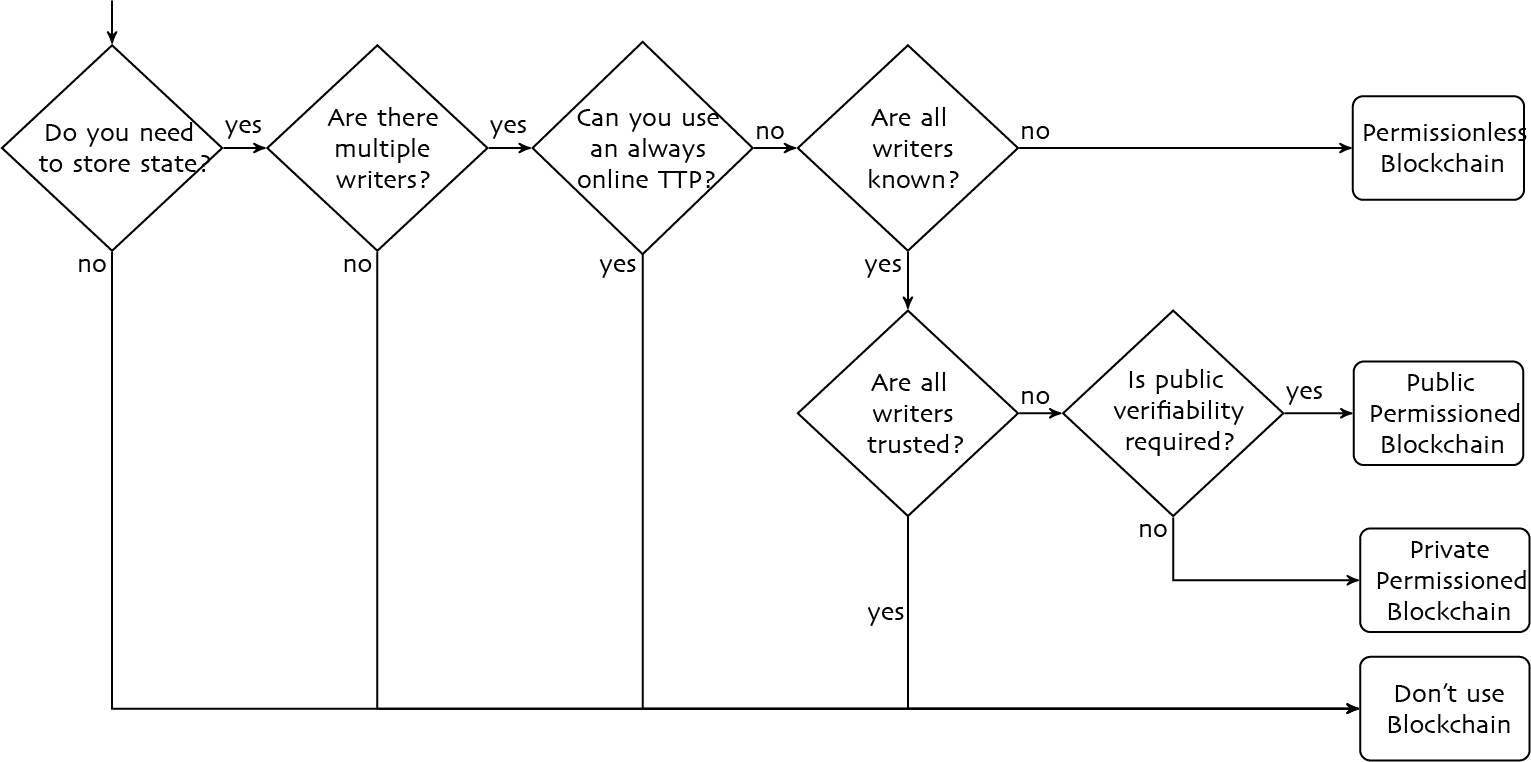
\includegraphics[scale=0.6]{Talk7/img/app/BCorNot}
	\end{center}
	\caption{Do you need a Blockchain?}
	\label{blockchain_or_not}
\end{figure}

\subsubsection{E-Voting}
The ability to vote is the very foundation of every successful democracy and must be accessible for all eligible citizens. Most common systems today are paper-based voting systems, have two major drawbacks.
\begin{enumerate}
	\item They do not scale very well
	\item They rely on the procedural security of officials conducting their jobs.
\end{enumerate}

Moreover, while various e-Voting systems exist, they all come with multiple security vulnerabilities, that lead to an enormous risk of election rigging and fraud.
The Blockchain, on the other hand, offers a transparent and incorruptible database that cannot have a single point of failure or be controlled by a single entity. It therefore immediately comes to mind when facing the above-stated problems. Meanwhile new questions of privacy and authenticating the writers arise.

Several systems exist up till today that make use of the blockchain technology. They all differ regarding the amount of integration and the role of the Blockchain. Different use cases either in theory or in practice have already been tested on smaller county elections or within private organizations. A quite exhaustive overview can be found in \cite{BenAyed2017}. According to \citeauthor{BenAyed2017} this system had the general problem, that single points of failure still existed and that critical parts of the code where closed.
Most existing systems such as Votebook(Source) or Vote Watchers(Source) still don't fully integrate the blockchain but instead use it as underlying database system in the form of a private permissioned blockchain. Those systems still rely on paper ballots. In this case, people have to authenticate by showing up in real life at a real-world voting booth, that uses the Blockchain for its tamper-proofness, its ability to account as an auditing system and because each voting booths results can be aggregated with all other stations to generate a final result in the end.
According to \citeauthor{Osgood2016}, these systems follow the only doable approach, as it doesn't deny the fact, that voters have to identify somewhere
Follow my Vote (Source) follows a fundamentally different approach, because it actually fully integrated the blockchains ability to act as a distributed ledger. Each voter installs a local "Voting Box" on his computer, authenticating via uploaded official documents through the organization that holds the election. Each voter requests ballot online and votes. Nevertheless, according to \citeauthor{Osgood2016}, this idea is fundamentally flawed as authentication mechanisms are still an issue and the technique could scare off remote voters.

Within all these systems, two fundamental questions seem to remain unanswered:
\begin{enumerate}
	\item \textbf{Authenticating users and the existence of a trusted third party}:    The writers of the blockchain are either directly or indirectly the voters themselves. To authenticate them, an organization that has all the data about them is necessary. In most cases, this leaves only the government as an option. However, according to the diagram by  \citeauthor{Wust2017} the use of Blockchain technology only makes sense if no trusted third party exists. Therefore, it is the role of the government that causes the dilemma itself. If the non-existing trust in the government is the justification for the use of the Blockchain, the question arises whether the government can be trusted regarding the authentication of the voters. Even though a systematic rigging is harder to achieve with this approach, the problem remains at hand.
	\item \textbf{The user as a single point of failure}: While the Blockchain does seem to be perfect for voting situations, its justification remains questionable. Especially, because it still leaves the most important point of failure unprotected: The user himself. Even the most tamper-proofed, blockchain-based voting system does not prevent hackers from a man-in-the-middle attack from a compromised end-device.
\end{enumerate}

Many of the desired e-Voting properties that the Blockchain technology provides have trade-offs. The aspect of how much privacy is granted to the voter is just one of many. On the other hand, no system has yet been proposed that has been shown to be secure, verifiable and private at the same time. The question of authentification comes into play as an additional point of failure of the concept.
Therefore, if an online trusted third party exists, the use of the blockchain is not necessary. If the government is trusted as far as the authentification of the voters goes, a public permissioned Blockchain can be a good fit. However, the security of the system then relies on the integrity of the validators.
If the government is trusted not at all, there exists no solution that overcomes that systematic flaw in a countries governance.

The Blockchain can, therefore, be a solution if the question of authentification can be answered satisfactorily. Otherwise, a traditional paper-based voting system is as good as any voting system including Blockchain based systems or systems that base on a trusted third party.

\subsubsection{Autonomous Vehicles, Smart Cities \& IoT}
Smart vehicles are increasingly connected to infrastructure via the Internet, thus making them part of the IoT. This development brings apparent advantages, but also many challenges, especially in the area of cybersecurity. Malicious attacks on a vehicle endanger not only the vehicles data and the passengers of the vehicle itself but also other road users. Also, while many common security and privacy methods exist to reduce the risk of an attack, they tend to be ineffective due to centralization, unscalability, and unsecured communication architectures \cite{DorriSteger2017}.
Meanwhile, the challenges on a secure and yet scalable system for connecting self-driving vehicles with other infrastructure are many: They need to be scalable, secure and tamper-proof, private but at the same time accessible to specific entities, such as traffic management systems or insurance.

The Blockchain offers solutions by design to many of the before mentioned problems. Therefore various approaches exist to connect self-driving vehicles with a blockchain-based architecture.

\citeauthor{DorriSteger2017}, propose a decentralized privacy-preserving and secure blockchain-based architecture for the smart vehicle ecosystem. It bases on its own Blockchain (Lightweight Scalable Blockchain) that minimizes the overhead and increases scalability as well as the throughput.
It consists of clusters of nodes which are connected to the system via Overlay Block Managers (OBMs).  All Transactions are broadcast to and verified by the OBMs. Each vehicle is connected to an overlay consisting of various OBMs that form the nodes of the Blockchain based system.
To ensure the user's privacy, each vehicle is equipped with internal vehicle storage to store sensitive data. It is the vehicle owner himself then, who defines which data is provided to third parties and which data is not.
To make specific Public Keys identifiable in the real world, a trusted third party is involved, and a centralized mechanism is used. This is needed in the case of service centers and software providers.
Many standard applications such as remote software updates, vehicle insurance, Smart Charging, and Vehicle Sharing Devices can be made possible through the use of the ecosystem.

Another approach is presented by \citeauthor{Rowan2017}: Their paper focusses on the communication between two road members through side-channels such as visible light and acoustic signals. To solve the problem of the limited data throughput while trying to securely validate the other communication partner, centralized approaches were discarded due to the high number of manufacturers and standards. Instead, a blockchain based domain name system is proposed. This way of exchanging identity information was chosen as the most promising way of storing public keys due to its robustness and security regarding large scale attacks.

The communication when two, e.g. vehicles meet each other needs to be extremely fast and include as little overhead as possible and work in the absence of any wireless or any centralized infrastructure. To make this possible, the handshake, that authenticates the involved partners and establishes a secure session, makes use of the Blockchain in the form of a decentralized Domain Name Service.
In this case, the Blockchain is used as a way to replace the need for a central authority when authenticating another vehicle. By creating a decentralized Name Service that binds the license plate value and identity together with a certificate, it is able to create a good base for a secure session between two verifiably trusted vehicles.

\citeauthor{Sharma2017} proposes a hierarchical system. At the top there exist two trusted third parties that register the vehicles (e.g., Department of Motor Vehicles) and that categorize the vehicles into miner nodes and ordinary nodes (Revocation Authority). Both parties exchange information with each other and the blockchain network consisting of the controller nodes. The controller nodes form the blockchain overlay at the top as they hold the information of the vehicle network and share it in a distributed manner with other controller nodes.
The next layer of the blockchain overlay is made by the miner nodes. Miner nodes are chosen vehicles that store data generated by sensors and applications. The top network supports the sharing of information between members of the blockchain network and is allowed to make specific data requests to the miner nodes, to gather information from sensors, etc.

The approach presented by \citeauthor{Sharma2017} is the only approach so far that thinks far beyond the incorporation of the blockchain into autonomous vehicles: It presents a framework for the controlled and secured interaction between all kinds of IoT devices. Cars as a particular case, are just one of them. The approach is very generally described, and the exact mechanisms that include the blockchain are not yet beyond an explanatory stage.
The idea though of having multiple layers of nodes that all incorporate the blockchain, but have different rights to access it, seems very promising and suits well to the hierarchical structures that are necessary to organize a smart city network. In some way, it can be thought of a system of checks and balances where some nodes have more rights, but their actions can always be seen and verified from everywhere at any time.
Again though, even though the Blockchain is presented as a central agent, various central authorities remain necessary if the digital has to be linked with the real world.


Applying the flow-chart by \citeauthor{Wust2017}, we run into the same problems as before. The main issue is whether a trusted third party exists and what its role is. Whether it exists explicitly such as in the systems of \cite{Sharma2017} or implicitly such as in the case of \cite{Rowan2017} or \cite{DorriSteger2017}, we always have a third party that comes into play. Whether it is trusted or not is another matter.
Having a trusted third party in play can only need to two different outcomes: Either, the use of the blockchain is not necessary, or a private permissioned blockchain should be chosen \cite{Wust2017}.
The only real advantage the blockchain offers, in this case, is its tamperproofness and its transparency. Hence all the advantages it offers, are the advantages of a decentral database system.

The idea to run a smart city IoT network on the blockchain suggests itself.
However, by looking at the problems that an IoT network for autonomous vehicles faces, we can not identify a single problem that would make the use of the blockchain absolutely necessary. Forcing the blockchain onto such problems always leads to the same result: A private permissioned blockchain that is stripped off its real (decentral) powers in order to be controllable and easy to use. Therefore it is nothing else than another form of a database, that could be replaced with any other database architecture.

\subsubsection{Personal Data Protection and Sharing in the medical sector}
No field is more torn between data sharing and data protection like the medical sector. One one hand, sharing private data is necessary to ensure safe medication and even save lives; on the other hand, the data is extremely sensitive and can inflict big problems on individuals if made public.

In the health-care sector three traditional models exist to deal with the facility of interoperability of medical data \cite{Kshetri2017}:
\begin{itemize}
	\item Push model: Medical information is sent from one provider to another
	\item Pull model: A provider asks another provider for information
	\item View model: A provider looks at another providers record.
\end{itemize}
A major drawback to all of these models is that the data is not audited or tracked in a standardized way. For example, if a patient is transferred to a different hospital, the new hospital may not be able to access data that was not "pushed." This lack of audit trail means that there is no guarantee of data integrity from the point where data is generated to the point where it is used.
It is argued by \cite{Kshetri2017} that the blockchain offers a fourth model, which makes it possible to share medical records securely across providers during the lifetime of a patient without having the need to include a trusted third party into the process. It leaves the data owner in full control about what is shared and leaves a verifiable audit trail of the data behind.

The combination of IoT and the Blockchain in the healthcare sector is particularly compelling. With the use of smart contracts, IoT devices carry out autonomous transactions on the Blockchain, while guaranteeing access control and data validity at the same time. Based on these thoughts various products and concepts have been created to make use of the Blockchain.


MedRec by \citeauthor{Azaria2016}:
The MedRec system is a sophisticated network to share and protect clinical data using the blockchain and smart contracts. Via smart contracts on an Ethereum blockchain they log patient-provider relationships that associate a medical record with viewing permissions and data retrieval instructions of execution on external databases.
Providers can add new records associated with a particular patient and patients can authorize the sharing of records between providers. The involved parties are notified by automated notifications when changes occur, or new data is added.
To avoid unintended or abusive use of data, different policies (set of rules) are put in place by the owner and carried out by smart contracts

The systems nodes consist of providers, that require a full server and database infrastructure, and patients, that can use any mobile device or web-interface and use only a local database with their own data.
To create incentives to run a blockchain node, MedRec offers block rewards and anonymized patient data.


\citeauthor{Cao2019} point out, that existing schemes cannot ensure the correctness and integrity of outsourced medical records. Especially not in the case, when authorized doctors collude with the cloud server to modify outsourced records which are generated by the doctors themselves.

To answer these problems, \citeauthor{Cao2019} propose a secure cloud-based system, that ensures the confidentiality, correctness, and integrity of outsourced medical records without introducing any trusted third party.
The proposed system works in the following way: Each patient makes an appointment with the hospital and obtains a treatment key for diagnosis. With the treatment key, a secure channel between patient and hospital and the doctors is established.
Before the treatment time, the patient generates warrants to delegate to doctors, that indicate the identities of the treating doctors for specific treatment time and other auxiliary information.
During the treatment time, doctors generate medical records for the patient: In the multi-doctor use-case, medical records are successively generated by all treating doctors based on the record by the previous doctor. In such a case a doctor is not only responsible for his own data, but also for the records his predecessors have generated.
The security of this system relies on the security of the Ethereum blockchain and the secure session established based on the treatment key. It is therefore protected against medical record modification attacks, impersonation attacks and a change of timeline whether by a hacker or an insider like a doctor.

Even though this approach is far less extensive than the MedRec approach, it does ensure the secure dealing of medical records through patients and doctors and provides the mechanisms to prevent any forging or tampering with the data through authenticated or unauthenticated people.

The only critical point that challenges the use of the blockchain is the question "Are all writers trusted?"\cite{Wust2017}. It leads to the  problem that it is the transitioning part of the whole process, the moment when the real world gets projected by a human being onto the digital world, that imposes the vulnerability.
If we do not trust the doctors to create rightful medical records, why do we consult them? Moreover, if we do trust them, why do we need a mechanism that prevents the doctors from forging medical records?

Disregarding of this fundamental problem, the system does provide proper security mechanisms against impersonation attacks and forgery that are undoubtedly useful and an improvement that is produced by the nature of the blockchain itself.
The question whether such a system must be run on the blockchain can therefore not be answered finally. The Blockchain is used to make the system more secure, Yes, but the blockchain cannot take over the responsibility for human or institutional malevolence.


The whole field of IoT devices also spreads into the direction of so-called Wireless Body Area Networks (WBANs). In a WBAN a patient is equipped with one or multiple wearables or implanted medical devices that take real-time measurements of vital indicators, such as heart rate or glucose levels. All devices report to one master device that collects and aggregates the data and offers a user-friendly interface.
The hereby existing security concerns are at hand: Live patient data is a lucrative target for hackers and poses not only a threat to the patient's health itself, but also to the privacy of its data.

To address these concerns, \citeauthor{Baccarini2018} propose integrating WBAN systems with smart contracts on a consortium-managed blockchain in order to provide a distributed data processing service, that creates an immutable log of the transactions between WBAN devices and the health care providers. This system allows for automatic notifications of health events to medical professionals in real time and in a secure manner.
In the presented system, the patient wears health monitor devices prescribed an applied by a doctor. The raw data of all devices gets collected and aggregated on a smartphone or a tablet and is then, together with customized threshold variables, sent to a specific smart contract on the blockchain. The smart contract evaluates the data and issues alerts to both patient and healthcare provider, as well as automated treatment instructions to the actuator nodes, if necessary.
No medical information is stored on the blockchain or in the smart contract. Instead, the only record that gets stored is the success of the transaction itself. The data itself is forwarded to a designated storage database. In the same way, all treatment commands from the smart contract and healthcare provider will be recorded as complete in the blockchain.
To authenticate the data later and to prevent and detect alterations, whether on purpose or accident, the blockchain transactions can be linked to the storage base where the patient's medical history lies.
The system is based on a private and consortium-led blockchain, consisting of healthcare companies, which allows only designated members to read the blocks, execute smart contracts or verify new blocks.

Compared with traditional systems, the blockchain based system offers higher performance regarding the availability, the immutability, privacy and transparency of the data  all due to the blockchains design. Regarding confidentiality and speed, the proposed system performs worse or equal than traditional systems.
The most considerable challenge of the system is maintaining security at every individual node. Because the traffic of the master device of the WBAN is routed via the user's internet connection, the data is possibly transferred over an open channel.  Other challenges are key management on a large scale and the block verification times when the alert issued by the smart contract takes too long.

This system by \cite{Baccarini2018} fundamentally differs from the others in one aspect: The initially generated data is generated by an IoT device and is per se, digital. No translation step happens between the generation and the incorporation of the data.
The use of the blockchain as the underlying system, therefore, makes a lot of sense, as it does not just use the blockchain architecture as a replacement for any kind of database, but - especially in the combination with the smart contract - to a real entity that supports the interconnection of IoT devices with the service provider in a distributed, secure and tamper-proof manner. The fact that it does not use the blockchain to actually store data, but only to log the transitions emphasized this aspect.

In our opinion, the system by \citeauthor{Baccarini2018} is the only approach that has a real use for the design of the blockchain, without trying to alter its nature. Also according to \citeauthor{Wust2017}, the permissioned private blockchain is the right choice, to create maximum privacy, while at the same time distributing the data securely to the right place at the right time.

An uncovered topic in all the work on the blockchain in the medical sector is the right to forget, as granted by the GDPR \cite{EuropeanCommission2017}. This fundamental right of a person to make records disappear is a big problem once a record is in the blockchain. At least from a theoretical point of view, a traditional system allows the deletion of a record. Meanwhile, a blockchain based system does per design not make it possible to delete anything at all, as it is stored within the chain, in an unmodifiable way. In this regard, the papers of \cite{Cao2019} and \cite{Azaria2016}, that really store data on the blockchain itself, have to be treated as approaches that violate the GDPR.

\subsubsection{Concluding remarks}
The covered topics show a broad use of the blockchain in order to increase a systems security. Most of the time the blockchain is chosen as a way to store data in a tamperproof manner and to be able to verify the integrity of the data at all times.
Most approaches, however, be it for reasons of following the trend or other reasons, do not take the blockchain for what it is, and instead try to create a suitable database system, that suits their use-case best reducing it to another way of storing data in a distributed way. The result is always a private permissioned blockchain that has no real solution for the initial problem: The incorporation of the data itself into the blockchain. The human as the first actor and the problem that arise with this fact, namely that we cannot outsource trust to a machine, is neglected.

Promising, on the other hand, are use cases where such a human translation-factor does not exist per se. Use-cases that already have that kind of data at hand that suits a blockchain scenario. Such approaches can exploit the advantages and properties of the blockchain technology at its fullest, without twisting it to fit a specific purpose.
Therefore, if the blockchain is able to act as its own entity, that in an "intelligent" way - through the use of e.g. smart contracts - is allowed to do what it can best, namely act on its own, distributing data in a secure and tamperproof way and secure it forever, the approach has a huge potential.



\newpage
\section{Final Considerations}

\begin{itemize}
  \item provide an overview of the section structure and contents (filler)
\end{itemize}

\subsection{Summary}

\begin{itemize}
  \item Length: around 1 page
  \item shortly summarize the overall work
  \item show the main thesis
\end{itemize}

\subsection{Discussion}

\begin{itemize}
  \item Length: around 1 page
  \item discuss any open questions about the contents
\end{itemize}

\subsection{Outlook}

\begin{itemize}
  \item Length: around 1 page
  \item describe possible topics of further research
\end{itemize}



\nocite{*}
\bibliographystyle{ieeetr}
\bibliography{Talk7/library}
